\documentclass{article}
\usepackage{tikz}
\usetikzlibrary{calc, shapes.arrows}

\begin{document}

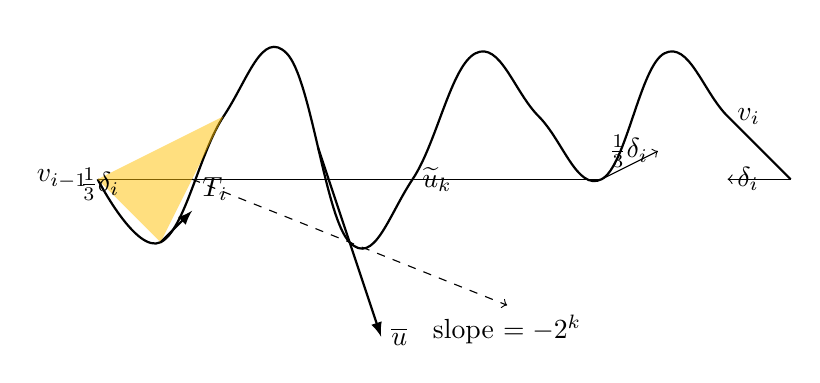
\begin{tikzpicture}[scale=0.8]
  % Define coordinates
  \coordinate (A) at (-3, 0);
  \coordinate (B) at (-2, -1);
  \coordinate (C) at (-1, 1);
  \coordinate (D) at (0, 2);
  \coordinate (E) at (1, -1);
  \coordinate (F) at (2, 0);
  \coordinate (G) at (3, 2);
  \coordinate (H) at (4, 1);
  \coordinate (I) at (5, 0);
  \coordinate (J) at (6, 2);
  \coordinate (K) at (7, 1);
  \coordinate (L) at (8, 0);
  
  % Draw the base line
  \draw (A) -- (I);
  
  % Draw the smooth function
  \draw[thick] plot [smooth, tension=.7] coordinates {(-3, 0) (-2, -1) (-1, 1) (0, 2) (1, -1) (2, 0) (3, 2) (4, 1) (5, 0) (6, 2) (7, 1) (8, 0)};
  
  % Draw the vertical dashed lines
  \draw[dashed] (A) -- ($(A)!1cm!(I)$);
  \draw[dashed] (I) -- ($(I)!1cm!(A)$);
  
  % Fill the orange triangle
  \fill[orange!50!yellow, opacity=0.5] (A) -- (B) -- (C) -- cycle;
  
  % Draw the arrows and labels
  \draw[-latex, thick] (B) -- ++(0.5, 0.5) node[above right] {$T_i$};
  \draw[-latex, thick] ($(D)!0.5!(E)$) -- ($(D)!1.5!(E)$) node[right] {$\overline{u}$};
  \draw[->, dashed] ($(B)!0.5!(C)$) -- ($(B)!0.5!(C)!2!(E)$) node[below] {slope $=-2^{k}$};
  \draw[->] (I) -- ($(I)!1cm!(K)$) node[left] {$\frac{1}{3}\delta_i$};
  \draw[->] (L) -- ($(L)!1cm!(I)$) node[right] {$\delta_i$};
  \node at (A) [left] {$v_{i-1}$};
  \node at (K) [right] {$v_i$};
  \node at (F) [right] {$\widetilde{u}_{k}$};
  
  % Mark the positions using nodes
  \node at ($(A)!0.5!(B)$) [above left] {$\frac{1}{3}\delta_i$};
\end{tikzpicture}

\small The estimate for $i \in {\cal J}_2$. From the fact that the value $v_{i-1}$ survives up to time $2^{-k}$, we deduce that the area of the yellow triangle can be controlled by the $L^1$ norm of all the $v_q^p$ in the interval $(x_{i-1}, x_i)$.